\documentclass[aspectratio=169]{beamer}
\usetheme{Madrid}
\usecolortheme{default}
\usepackage[utf8]{inputenc}
\usepackage[T5]{fontenc}
\usepackage{graphicx}
\usepackage{hyperref}
\usepackage{booktabs}
\usepackage{amsmath}
\usepackage{listings}
\usepackage{xcolor}

\setbeamertemplate{caption}[numbered]
\renewcommand{\figurename}{Hình}
\renewcommand{\thefigure}{7.\arabic{figure}}

% Cấu hình listings cho Python
\definecolor{codegreen}{rgb}{0,0.6,0}
\definecolor{codegray}{rgb}{0.5,0.5,0.5}
\definecolor{codepurple}{rgb}{0.58,0,0.82}
\definecolor{backcolour}{rgb}{0.95,0.95,0.92}

\lstdefinestyle{mystyle}{
    backgroundcolor=\color{backcolour},   
    commentstyle=\color{codegreen},
    keywordstyle=\color{magenta},
    numberstyle=\tiny\color{codegray},
    stringstyle=\color{codepurple},
    basicstyle=\ttfamily\footnotesize,
    breakatwhitespace=false,         
    breaklines=true,                 
    captionpos=b,                    
    keepspaces=true,                 
    numbers=left,                    
    numbersep=5pt,                  
    showspaces=false,                
    showstringspaces=false,
    showtabs=false,                  
    tabsize=2
}
\lstset{style=mystyle}

\title[Chương 7: Chuyên sâu Keras]{Học Sâu (Deep Learning) \\ \vspace{0.5cm} \Large Chương 7: Lập trình Chuyên sâu với Keras \\ (A Deep Dive on Keras)}
\author{Đại học Đông Á}
\date{\today}

\begin{document}

\begin{frame}
    \titlepage
\end{frame}

\begin{frame}{Nội dung chương}
    \tableofcontents
\end{frame}

\section{1. Triết lý Thiết kế của Keras}

\begin{frame}{Từng bước phơi bày sự phức tạp (Progressive Disclosure)}
    \begin{columns}
        \column{0.5\textwidth}
        \begin{itemize}
            \item \textbf{Nguyên tắc thiết kế Keras:} Làm cho mọi thứ trở nên dễ bắt đầu, nhưng vẫn hoàn toàn khả thi để xử lý các bài toán siêu phức tạp.
            \item Không có một "con đường duy nhất". Keras cung cấp một \textbf{Phổ quy trình (Spectrum of workflows)}.
            \item Các trường hợp đơn giản có thể được giải quyết bằng vài dòng mã, trong khi các công việc phức tạp có thể yêu cầu viết mã chi tiết.
        \end{itemize}
        
        \column{0.5\textwidth}
        \begin{figure}
            \centering
            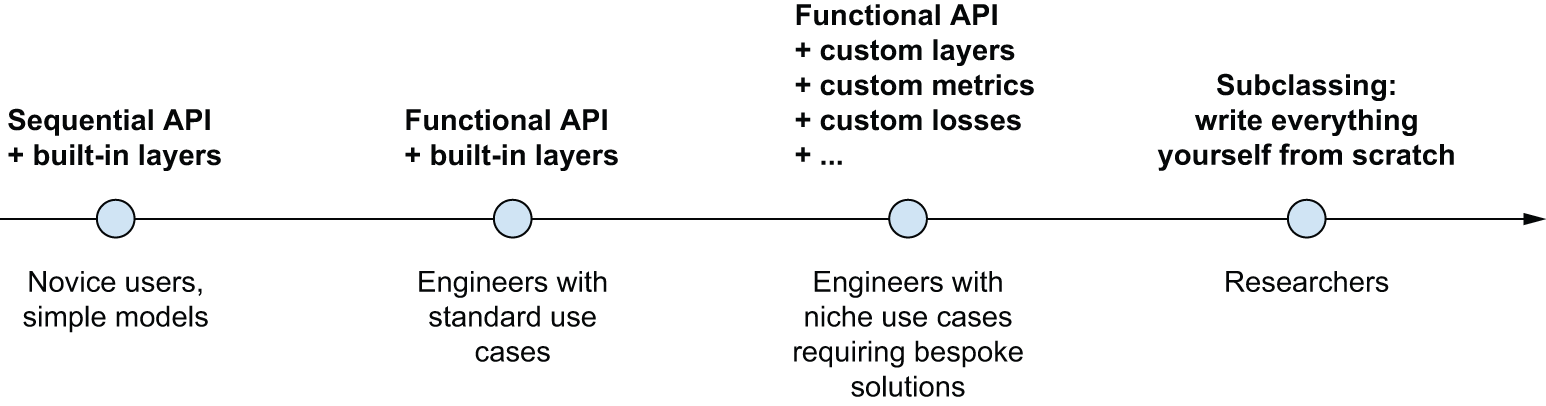
\includegraphics[width=\textwidth,height=0.7\textheight,keepaspectratio]{../../images/ch07/progressive_disclosure_of_complexity_models.f43bcdb0.png}
            \caption{Từ Sequential đến Model Subclassing}
        \end{figure}
    \end{columns}
\end{frame}

\begin{frame}{Spectrum of workflows (Phổ quy trình)}
    \begin{itemize}
        \item Keras được thiết kế giống như triết lý của Python: Đa mô hình (multi-paradigm).
        \item \textbf{Người mới (Beginner):} Sử dụng Keras như Scikit-learn (dùng \texttt{model.fit()}, \texttt{Sequential}).
        \item \textbf{Nhà nghiên cứu (Researcher):} Sử dụng Keras như NumPy/TensorFlow lõi (viết tay mọi thứ từ đầu bằng GradientTape).
        \item Đặc biệt, các API này \textbf{có thể giao tiếp trơn tru với nhau}. Một mô hình \texttt{Sequential} có thể được lồng vào một mô hình \texttt{Subclassing}.
    \end{itemize}
\end{frame}

\begin{frame}{Vòng lặp Tiến bộ (The Loop of Progress)}
    \begin{columns}
        \column{0.5\textwidth}
        \begin{itemize}
            \item Khoa học là quá trình thử nghiệm lặp đi lặp lại (Iterative Process).
            \item \textbf{Idea:} Khởi tạo ý tưởng.
            \item \textbf{Experiment:} Cài đặt mã nguồn.
            \item \textbf{Evaluate:} Đánh giá kết quả $\rightarrow$ Rút ra bài học và tạo Idea mới.
            \item Keras tối ưu hóa trải nghiệm người dùng (UX) để thu ngắn tối đa thời gian lập trình.
        \end{itemize}
        
        \column{0.5\textwidth}
        \begin{figure}
            \centering
            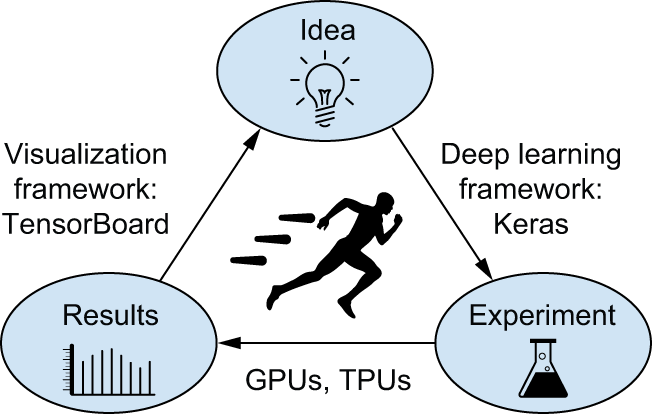
\includegraphics[width=\textwidth,height=0.7\textheight,keepaspectratio]{../../images/ch07/the_loop_of_progress.df126e89.png}
            \caption{Vòng lặp phát triển Mô hình ML}
        \end{figure}
    \end{columns}
\end{frame}

\section{2. Ba phương pháp Xây dựng Mô hình}

\begin{frame}{Phương pháp 1: Sequential API}
    \begin{itemize}
        \item Cấu trúc dữ liệu dạng \textbf{Danh sách (Python List)}.
        \item Đơn giản nhất, dễ tiếp cận nhất. Các lớp được xếp chồng tuyến tính (lớp sau nối tiếp lớp trước).
        \item \textbf{Hạn chế:} Chỉ áp dụng được cho mô hình 1 đầu vào, 1 đầu ra.
        \item Không thể áp dụng cho: Mô hình đa đầu vào (Multi-input), đa đầu ra (Multi-output), hay cấu trúc phân nhánh.
    \end{itemize}
\end{frame}

\begin{frame}[fragile]{Sequential API: Mã nguồn cơ bản}
Khởi tạo mô hình Sequential dưới dạng một danh sách (list):
\begin{lstlisting}[language=Python]
import keras
from keras import layers

model = keras.Sequential(
    [
        layers.Dense(64, activation="relu"),
        layers.Dense(10, activation="softmax"),
    ]
)
\end{lstlisting}
Hoặc xây dựng dần dần (incrementally) bằng hàm \texttt{add()}:
\begin{lstlisting}[language=Python]
model = keras.Sequential()
model.add(layers.Dense(64, activation="relu"))
model.add(layers.Dense(10, activation="softmax"))
\end{lstlisting}
\end{frame}

\begin{frame}[fragile]{Sequential API: Trọng số (Weights) và Shape}
Các lớp trong Keras chỉ tạo trọng số (build) khi biết kích thước đầu vào (input shape):
\begin{lstlisting}[language=Python]
>>> model.weights  # Before build
[]
>>> model.build(input_shape=(None, 3))
>>> model.weights  # Weights created
[<Variable shape=(3, 64) ...>, <Variable shape=(64,) ...>]
\end{lstlisting}
In bảng tóm tắt cấu trúc:
\begin{lstlisting}[language=Python]
>>> model.summary()
Model: "sequential_1"
...
\end{lstlisting}
\end{frame}

\begin{frame}[fragile]{Sequential API: Khai báo Input Shape trước}
Sử dụng đối tượng \texttt{Input} để khai báo đầu vào, cho phép mô hình được build tự động ngay từ đầu:
\begin{lstlisting}[language=Python]
model = keras.Sequential()
model.add(keras.Input(shape=(3,)))
model.add(layers.Dense(64, activation="relu"))

# Model is built automatically, we can call summary now
model.summary()
\end{lstlisting}
Điều này đặc biệt hữu ích khi thiết kế các mạng CNN sâu.
\end{frame}

\begin{frame}{Phương pháp 2: Functional API}
    \begin{itemize}
        \item Coi các layer là các \textbf{Hàm (Functions)}. Nhận Tensor và trả về Tensor.
        \item Cung cấp giải pháp linh hoạt hơn nhiều, cho phép xây dựng mạng \textbf{Đồ thị đa hướng (Directed Acyclic Graph)}.
        \item API phổ biến nhất trong thực tế. "Cảm giác như chơi lắp ráp LEGO".
        \item Cho phép định nghĩa nhiều luồng vào ra, chia nhánh đồ thị.
    \end{itemize}
\end{frame}

\begin{frame}[fragile]{Functional API: Các bước cơ bản}
\begin{lstlisting}[language=Python]
# 1. Define Input
inputs = keras.Input(shape=(3,), name="my_input")

# 2. Build graph by calling layers like functions
features = layers.Dense(64, activation="relu")(inputs)

# 3. Create outputs
outputs = layers.Dense(10, activation="softmax")(features)

# 4. Initialize Model with inputs and outputs
model = keras.Model(inputs=inputs, outputs=outputs, name="my_functional_model")
\end{lstlisting}
Đối tượng \texttt{inputs} là một \textbf{Symbolic Tensor} (Tensor ký hiệu), chỉ chứa thông tin shape và dtype, không chứa dữ liệu thực.
\end{frame}

\begin{frame}{Functional API: Ví dụ Mạng phân loại vé}
    \begin{columns}
        \column{0.5\textwidth}
        \begin{itemize}
            \item Hệ thống Ticket Classifier.
            \item \textbf{3 Đầu vào (Inputs):} 
            \begin{itemize}
                \item Tiêu đề (title)
                \item Nội dung (text\_body)
                \item Thẻ (tags)
            \end{itemize}
            \item \textbf{2 Đầu ra (Outputs):}
            \begin{itemize}
                \item Mức độ ưu tiên (priority: 0 đến 1)
                \item Phòng ban xử lý (department)
            \end{itemize}
        \end{itemize}
        
        \column{0.5\textwidth}
        \begin{figure}
            \centering
            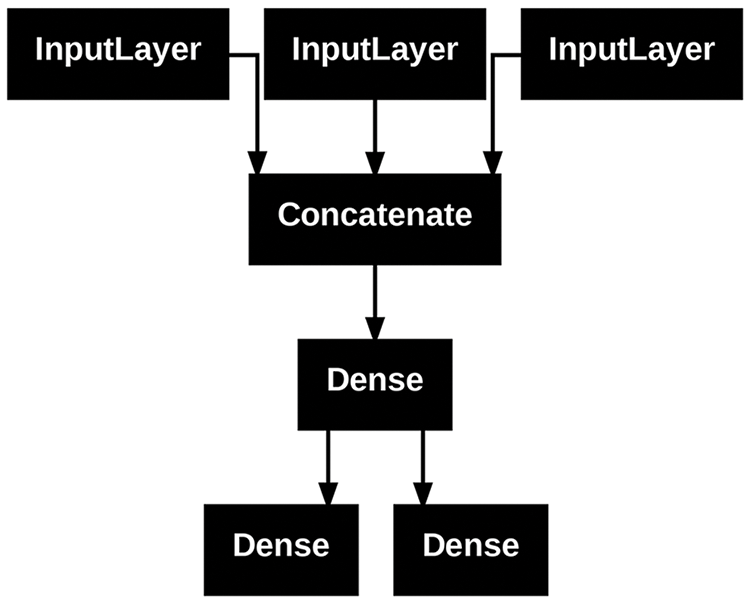
\includegraphics[width=\textwidth,height=0.7\textheight,keepaspectratio]{../../images/ch07/ticket_classifier.6d8d5711.png}
            \caption{Sơ đồ mạng đa luồng}
        \end{figure}
    \end{columns}
\end{frame}

\begin{frame}[fragile]{Functional API: Cài đặt hệ thống phân loại vé}
\begin{lstlisting}[language=Python, basicstyle=\ttfamily\scriptsize]
vocabulary_size = 10000
num_tags = 100
num_departments = 4

# Inputs
title = keras.Input(shape=(vocabulary_size,), name="title")
text_body = keras.Input(shape=(vocabulary_size,), name="text_body")
tags = keras.Input(shape=(num_tags,), name="tags")

# Concatenate features
features = layers.Concatenate()([title, text_body, tags])
features = layers.Dense(64, activation="relu", name="dense_features")(features)

# Outputs
priority = layers.Dense(1, activation="sigmoid", name="priority")(features)
department = layers.Dense(num_departments, activation="softmax", name="department")(features)

# Initialize Model
model = keras.Model(inputs=[title, text_body, tags], outputs=[priority, department])
\end{lstlisting}
\end{frame}

\begin{frame}[fragile]{Functional API: Huấn luyện với Multi-Input/Output}
Khi dùng \texttt{fit()}, bạn truyền Dữ liệu dạng List hoặc Dictionary:
\begin{lstlisting}[language=Python, basicstyle=\ttfamily\scriptsize]
model.compile(
    optimizer="adam",
    loss={
        "priority": "mean_squared_error",
        "department": "sparse_categorical_crossentropy",
    },
    metrics={"priority": ["mae"], "department": ["accuracy"]}
)

model.fit(
    {"title": title_data, "text_body": text_body_data, "tags": tags_data},
    {"priority": priority_data, "department": department_data},
    epochs=1
)
\end{lstlisting}
Sử dụng tên `name` của Input/Output (Dictionary mode) thường dễ bảo trì hơn so với truyền mảng (List mode).
\end{frame}

\begin{frame}{Functional API: Luồng dữ liệu và Hình dáng (Shapes)}
    \begin{columns}
        \column{0.5\textwidth}
        \begin{itemize}
            \item Có thể vẽ sơ đồ mạng bằng tiện ích \texttt{plot\_model}.
            \item Tham số \texttt{show\_shapes=True} in ra cả kích thước.
            \item TensorShape \texttt{(None, 10000)}: \texttt{None} đại diện cho kích thước Lô (Batch size) bất kì.
            \item Kiểm tra kích thước ở Design Time giúp loại bỏ các lỗi ma trận kích thước lệch pha (Shape Mismatch).
        \end{itemize}
        
        \column{0.5\textwidth}
        \begin{figure}
            \centering
            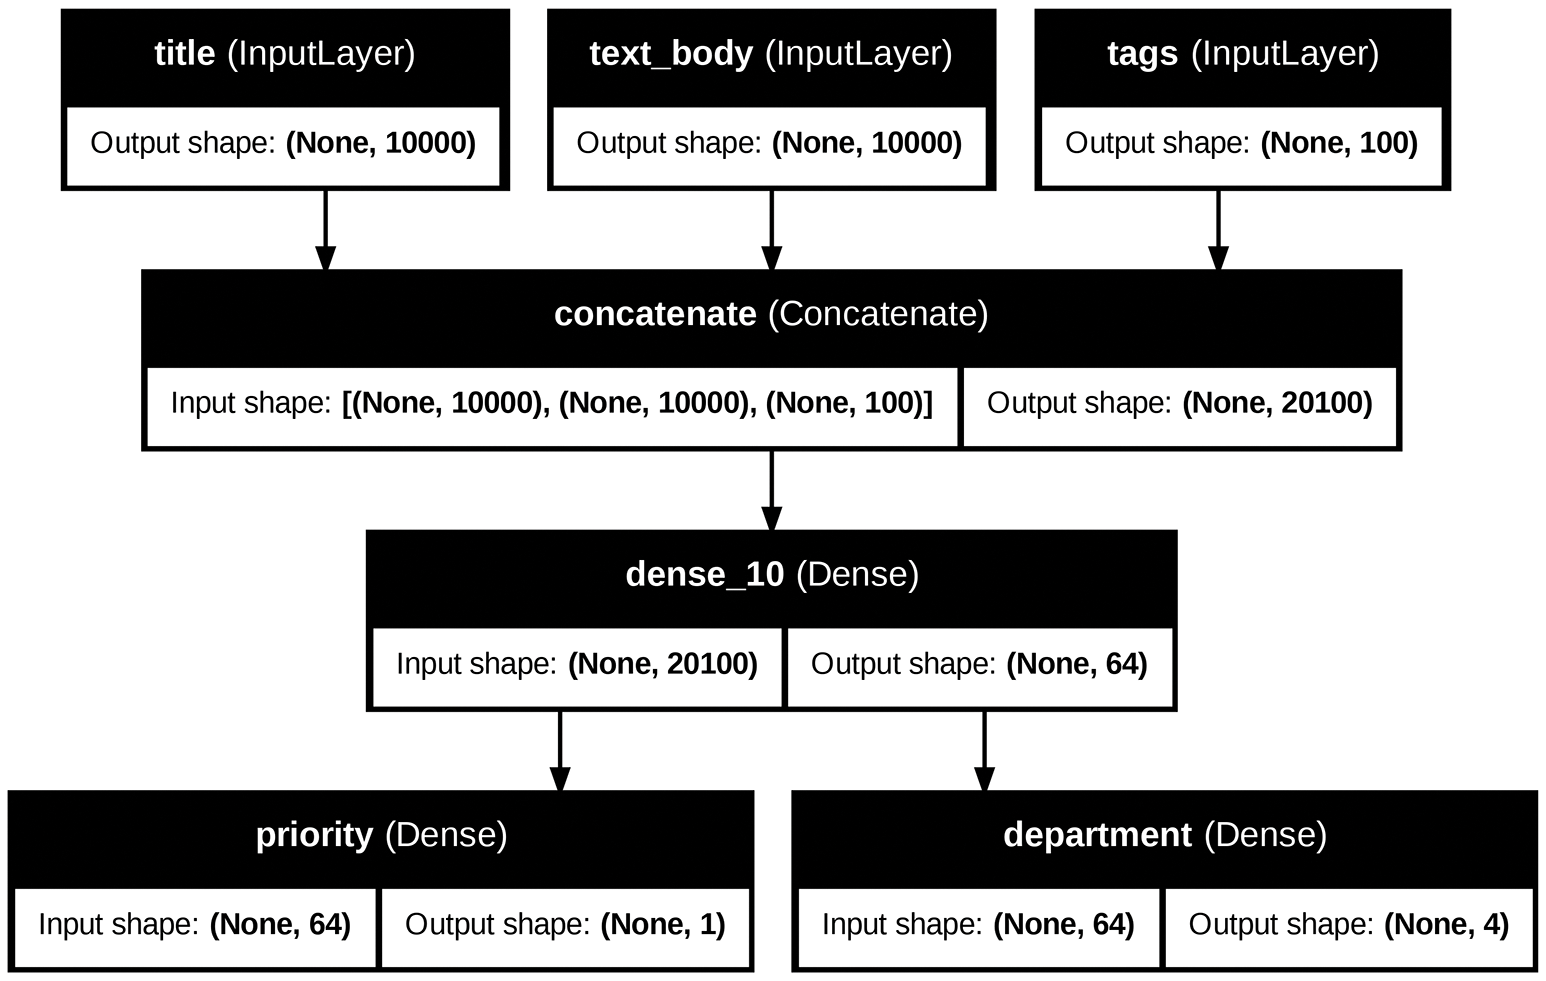
\includegraphics[width=\textwidth,height=0.7\textheight,keepaspectratio]{../../images/ch07/ticket_classifier_with_shapes.1c26af81.png}
            \caption{Đồ thị truyền tải Shapes}
        \end{figure}
    \end{columns}
\end{frame}

\begin{frame}[fragile]{Functional API: Trích xuất Tính năng (Feature Extraction)}
    \begin{columns}
        \column{0.5\textwidth}
        \begin{itemize}
            \item Mô hình chứa các \textit{nút trung gian (Intermediate Nodes)}. Ta có thể tái sử dụng chúng.
            \item Trích xuất layer tại mốc số 4 (Dense layer) và bổ sung 1 nhánh \texttt{difficulty} (độ khó).
        \end{itemize}
\begin{lstlisting}[language=Python, basicstyle=\ttfamily\tiny]
features = model.layers[4].output
difficulty = layers.Dense(
    3, activation="softmax", name="difficulty"
)(features)

new_model = keras.Model(
    inputs=[title, text_body, tags], 
    outputs=[priority, department, difficulty]
)
\end{lstlisting}
        
        \column{0.5\textwidth}
        \begin{figure}
            \centering
            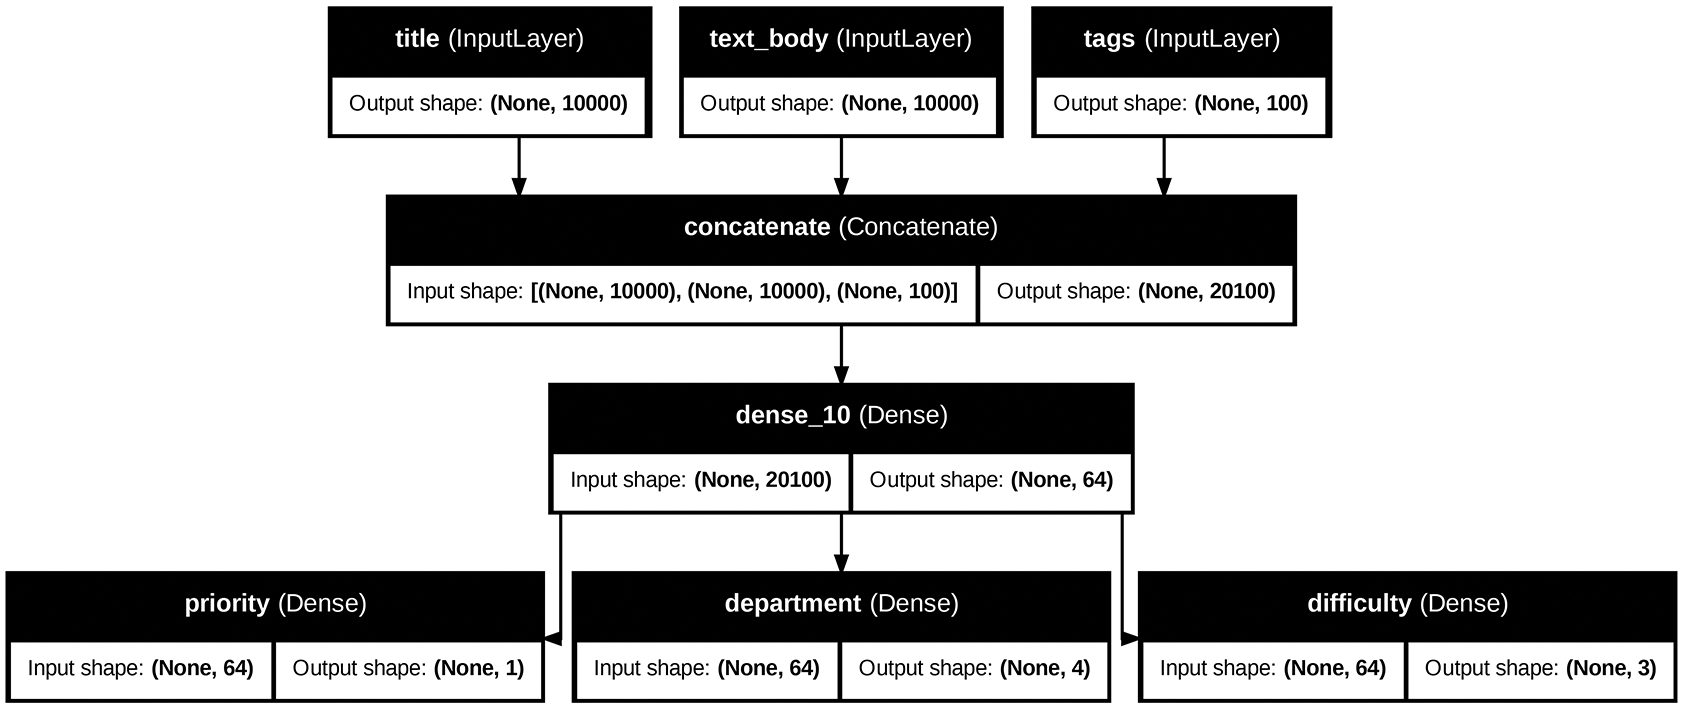
\includegraphics[width=\textwidth,height=0.65\textheight,keepaspectratio]{../../images/ch07/updated_ticket_classifier.d0baf1fe.png}
            \caption{Mở rộng đồ thị}
        \end{figure}
    \end{columns}
\end{frame}

\begin{frame}{Phương pháp 3: Model Subclassing}
    \begin{itemize}
        \item Phương pháp cấp thấp, linh hoạt nhất.
        \item Kế thừa trực tiếp Lập trình Hướng đối tượng (OOP) từ lớp \texttt{keras.Model}.
        \item Khai báo các Layer (chứa trọng số) tại hàm tạo \texttt{\_\_init\_\_()}.
        \item Định nghĩa dòng chảy Toán học ngầm (Forward pass) tại hàm \texttt{call()}.
        \item \textbf{Ưu điểm:} Cung cấp khả năng kiểm soát tuyệt đối, ví dụ sử dụng vòng lặp \texttt{for}, đệ quy bên trong mạng Nơ-ron.
    \end{itemize}
\end{frame}

\begin{frame}[fragile]{Model Subclassing: Mã nguồn}
Viết lại Ticket Classifier dưới dạng Class:
\begin{lstlisting}[language=Python, basicstyle=\ttfamily\scriptsize]
class CustomerTicketModel(keras.Model):
    def __init__(self, num_departments):
        super().__init__() # Always call parent constructor
        self.concat_layer = layers.Concatenate()
        self.mixing_layer = layers.Dense(64, activation="relu")
        self.priority_scorer = layers.Dense(1, activation="sigmoid")
        self.department_classifier = layers.Dense(num_departments, activation="softmax")

    def call(self, inputs): # Forward pass logic
        title = inputs["title"]
        text_body = inputs["text_body"]
        tags = inputs["tags"]
        
        features = self.concat_layer([title, text_body, tags])
        features = self.mixing_layer(features)
        priority = self.priority_scorer(features)
        department = self.department_classifier(features)
        return priority, department
\end{lstlisting}
\end{frame}

\begin{frame}{Model Subclassing: Cảnh báo}
    \begin{itemize}
        \item \textbf{Nhược điểm:} Bạn đang viết "mã byte" dạng hộp đen (Black-box), không còn là đồ thị (Graph) rõ ràng nữa.
        \item Không thể gọi hàm \texttt{summary()} để in ra cấu trúc các nút kết nối.
        \item Không thể sử dụng \texttt{plot\_model()} để vẽ ảnh cấu trúc mạng.
        \item Không thể dùng kĩ thuật \textbf{Feature Extraction} do không thể truy xuất \texttt{model.layers[i].output}.
        \item Người lập trình hoàn toàn chịu trách nhiệm cho các lỗi logic bên trong \texttt{call()}.
    \end{itemize}
\end{frame}

\section{3. Tùy biến Vòng lặp Huấn luyện (Customizing)}

\begin{frame}{Tùy biến Keras: Khi các hàm có sẵn là không đủ}
    \begin{itemize}
        \item API \texttt{model.fit()} rất tốt cho hầu hết bài toán thực tế.
        \item Nhưng với các nhà nghiên cứu, họ thường phát minh ra các hàm Mất mát (Losses) mới, thước đo (Metrics) mới, hoặc những thuật toán Huấn luyện phi tiêu chuẩn (GANs).
        \item Keras cho phép ghi đè hoàn toàn:
        \begin{itemize}
            \item Custom Loss
            \item Custom Metric
            \item Custom Training Step (\texttt{train\_step()})
            \item Custom Training Loop (Low-level GradientTape)
        \end{itemize}
    \end{itemize}
\end{frame}

\begin{frame}[fragile]{Tự định nghĩa Hàm Mất mát (Custom Losses)}
Đôi khi hàm \textit{Mean Squared Error (MSE)} mặc định là không đủ. Ta có thể viết một hàm (function) đơn giản:
\begin{lstlisting}[language=Python]
import tensorflow as tf

def custom_mean_squared_error(y_true, y_pred):
    return tf.reduce_mean(tf.square(y_true - y_pred))

model.compile(optimizer="adam", loss=custom_mean_squared_error)
\end{lstlisting}

Hoặc kế thừa lớp \texttt{keras.losses.Loss}:
\begin{lstlisting}[language=Python]
class CustomMSE(keras.losses.Loss):
    def __init__(self, name="custom_mse", **kwargs):
        super().__init__(name=name, **kwargs)

    def call(self, y_true, y_pred):
        return tf.reduce_mean(tf.square(y_true - y_pred))
\end{lstlisting}
\end{frame}

\begin{frame}{Tự định nghĩa Thước đo (Custom Metrics)}
    Metrics khác với Loss ở chỗ nó mang \textbf{Trạng thái (Stateful)}. 
    \begin{itemize}
        \item Loss: Tính cục bộ trên mỗi Batch (Lô).
        \item Metric: Phải cộng dồn trên nhiều Batch và tính trung bình trong suốt 1 Epoch.
        \item Kế thừa lớp \texttt{keras.metrics.Metric} yêu cầu 3 hàm:
        \begin{enumerate}
            \item \texttt{update\_state()}: Cộng dồn kết quả đếm cho mỗi Batch.
            \item \texttt{result()}: Tính toán và trả về kết quả hiển thị cho người dùng.
            \item \texttt{reset\_state()}: Xóa sạch bộ đếm về 0 khi bắt đầu một Epoch mới.
        \end{enumerate}
    \end{itemize}
\end{frame}

\begin{frame}[fragile]{Custom Metrics: Cài đặt thực tế (Root Mean Squared Error)}
\begin{lstlisting}[language=Python, basicstyle=\ttfamily\scriptsize]
class RootMeanSquaredError(keras.metrics.Metric):
    def __init__(self, name="rmse", **kwargs):
        super().__init__(name=name, **kwargs)
        # Declare state variables
        self.mse_sum = self.add_weight(name="mse_sum", initializer="zeros")
        self.total_samples = self.add_weight(name="total_samples", initializer="zeros")

    def update_state(self, y_true, y_pred, sample_weight=None):
        mse = tf.reduce_mean(tf.square(y_true - y_pred))
        self.mse_sum.assign_add(mse)
        self.total_samples.assign_add(1.0)

    def result(self):
        # Return sqrt of accumulated mean MSE
        return tf.sqrt(self.mse_sum / self.total_samples)

    def reset_state(self):
        self.mse_sum.assign(0.)
        self.total_samples.assign(0.)
\end{lstlisting}
\end{frame}

\begin{frame}{Viết lại Vòng lặp Huấn luyện với GradientTape}
    Thay vì gọi \texttt{model.fit()}, ta có thể sử dụng \texttt{tf.GradientTape} để tự điều khiển phép tính \textbf{Đạo hàm riêng (Backpropagation)}:
    \begin{equation}
        \Delta W = - \eta \cdot \frac{\partial L}{\partial W}
    \end{equation}
    Quy trình 4 bước của 1 Batch (Lô dữ liệu):
    \begin{enumerate}
        \item Mở không gian bộ nhớ (Tape), truyền dữ liệu qua Mạng.
        \item Tính toán Loss $L$.
        \item Dùng Tape truy xuất Gradient $\frac{\partial L}{\partial W}$ của các Trọng số.
        \item Gửi Gradient cho Trình tối ưu hóa (Optimizer) để cập nhật Trọng số $W$.
    \end{enumerate}
\end{frame}

\begin{frame}[fragile]{Custom Training Loop: Mã nguồn GradientTape}
Đây là kiến thức quan trọng nhất dành cho một Chuyên gia Học sâu.
\begin{lstlisting}[language=Python, basicstyle=\ttfamily\scriptsize]
optimizer = keras.optimizers.Adam(learning_rate=1e-3)
loss_fn = keras.losses.SparseCategoricalCrossentropy()

for epoch in range(3): # Epoch loop
    for step, (x_batch, y_batch) in enumerate(train_dataset): # Batch loop
        # 1. Open Tape
        with tf.GradientTape() as tape:
            # 2. Feed-forward and calculate loss
            logits = model(x_batch, training=True) 
            loss_value = loss_fn(y_batch, logits)
            
        # 3. Compute Gradients
        gradients = tape.gradient(loss_value, model.trainable_weights)
        
        # 4. Apply Gradients (Update weights)
        optimizer.apply(gradients, model.trainable_weights)
\end{lstlisting}
\end{frame}

\begin{frame}[fragile]{Ghi đè hàm \texttt{train\_step()}}
Để kết hợp vòng lặp thủ công với tính năng của \texttt{fit()} (hiển thị thanh tiến trình), bạn có thể ghi đè \texttt{train\_step()}:
\begin{lstlisting}[language=Python, basicstyle=\ttfamily\scriptsize]
class CustomModel(keras.Model):
    def train_step(self, data):
        inputs, targets = data
        with tf.GradientTape() as tape:
            predictions = self(inputs, training=True)
            loss = self.compute_loss(y=targets, y_pred=predictions)

        gradients = tape.gradient(loss, self.trainable_weights)
        self.optimizer.apply(gradients, self.trainable_weights)

        # Update Metrics
        for metric in self.metrics:
            if metric.name == "loss":
                metric.update_state(loss)
            else:
                metric.update_state(targets, predictions)
        return {m.name: m.result() for m in self.metrics}
\end{lstlisting}
Bạn vẫn có thể dùng `model.fit()` và tận hưởng mọi Callback.
\end{frame}

\section{4. Callbacks: Tự động hóa quá trình Huấn luyện}

\begin{frame}{Sức mạnh của Callbacks}
    \begin{itemize}
        \item Huấn luyện mô hình Deep Learning có thể tốn hàng giờ hoặc nhiều tuần.
        \item Bạn không thể cứ ngồi nhìn màn hình suốt quá trình đó để can thiệp kịp thời.
        \item \textbf{Callbacks} là các "hook" (chốt chặn) được kích hoạt tự động vào các thời điểm cụ thể (Đầu/cuối Epoch, Đầu/cuối Batch).
        \item \textbf{Ứng dụng:} Tự dừng sớm, Lưu trọng số, Thay đổi tốc độ học...
    \end{itemize}
\end{frame}

\begin{frame}[fragile]{Các Callbacks tích hợp: EarlyStopping \& ModelCheckpoint}
\textbf{EarlyStopping:} Tự động dừng huấn luyện khi \texttt{val\_loss} không còn giảm (Ngăn Overfitting).
\textbf{ModelCheckpoint:} Tự động sao lưu Trọng số Tốt nhất xuống ổ cứng.

\begin{lstlisting}[language=Python, basicstyle=\ttfamily\scriptsize]
callbacks_list = [
    keras.callbacks.EarlyStopping(
        monitor="val_accuracy", 
        patience=2, # Stop if no improvement after 2 epochs
    ),
    keras.callbacks.ModelCheckpoint(
        filepath="my_checkpoint.keras",
        monitor="val_loss",
        save_best_only=True, # Only save model with lowest val_loss
    )
]
model.fit(..., callbacks=callbacks_list, ...)
\end{lstlisting}
\end{frame}

\begin{frame}[fragile]{Tùy biến Callback (Custom Callback)}
Bạn có thể tự tạo Callback bằng cách kế thừa \texttt{keras.callbacks.Callback}.
Các hàm sự kiện bạn có thể ghi đè:
\begin{lstlisting}[language=Python, basicstyle=\ttfamily\scriptsize]
class MyCustomCallback(keras.callbacks.Callback):
    def on_epoch_begin(self, epoch, logs=None):
        print(f"Start epoch {epoch}")
        
    def on_epoch_end(self, epoch, logs=None):
        print(f"End epoch {epoch}")
        
    def on_batch_begin(self, batch, logs=None): ...
    def on_batch_end(self, batch, logs=None): ...
    def on_train_begin(self, logs=None): ...
    def on_train_end(self, logs=None): ...
\end{lstlisting}
\end{frame}

\begin{frame}[fragile]{Custom Callback: Ví dụ ghi lại Loss theo Batch}
\begin{lstlisting}[language=Python, basicstyle=\ttfamily\scriptsize]
import matplotlib.pyplot as plt

class LossHistory(keras.callbacks.Callback):
    def on_train_begin(self, logs=None):
        self.per_batch_losses = [] # Store loss for every batch

    def on_batch_end(self, batch, logs=None):
        self.per_batch_losses.append(logs.get("loss"))

    def on_train_end(self, logs=None):
        plt.clf()
        plt.plot(range(len(self.per_batch_losses)), self.per_batch_losses, label="Training loss")
        plt.xlabel(f"Batchs (Total: {len(self.per_batch_losses)})")
        plt.ylabel("Loss")
        plt.legend()
        plt.savefig("loss_history_callback_example.png")
\end{lstlisting}
\end{frame}

\begin{frame}{Kết quả sinh ra bởi Custom Callback}
    \begin{columns}
        \column{0.5\textwidth}
        \begin{itemize}
            \item Mật độ dày đặc của biểu đồ cho thấy sự thay đổi Loss ở cấp độ Lô (Batch-level) (Thay vì mức Epoch).
            \item Đây là một phương pháp kiểm tra (sanity-check) xuất sắc để xem dữ liệu có thực sự "nhạy" với bước học của mạng Nơ-ron hay không.
        \end{itemize}
        
        \column{0.5\textwidth}
        \begin{figure}
            \centering
            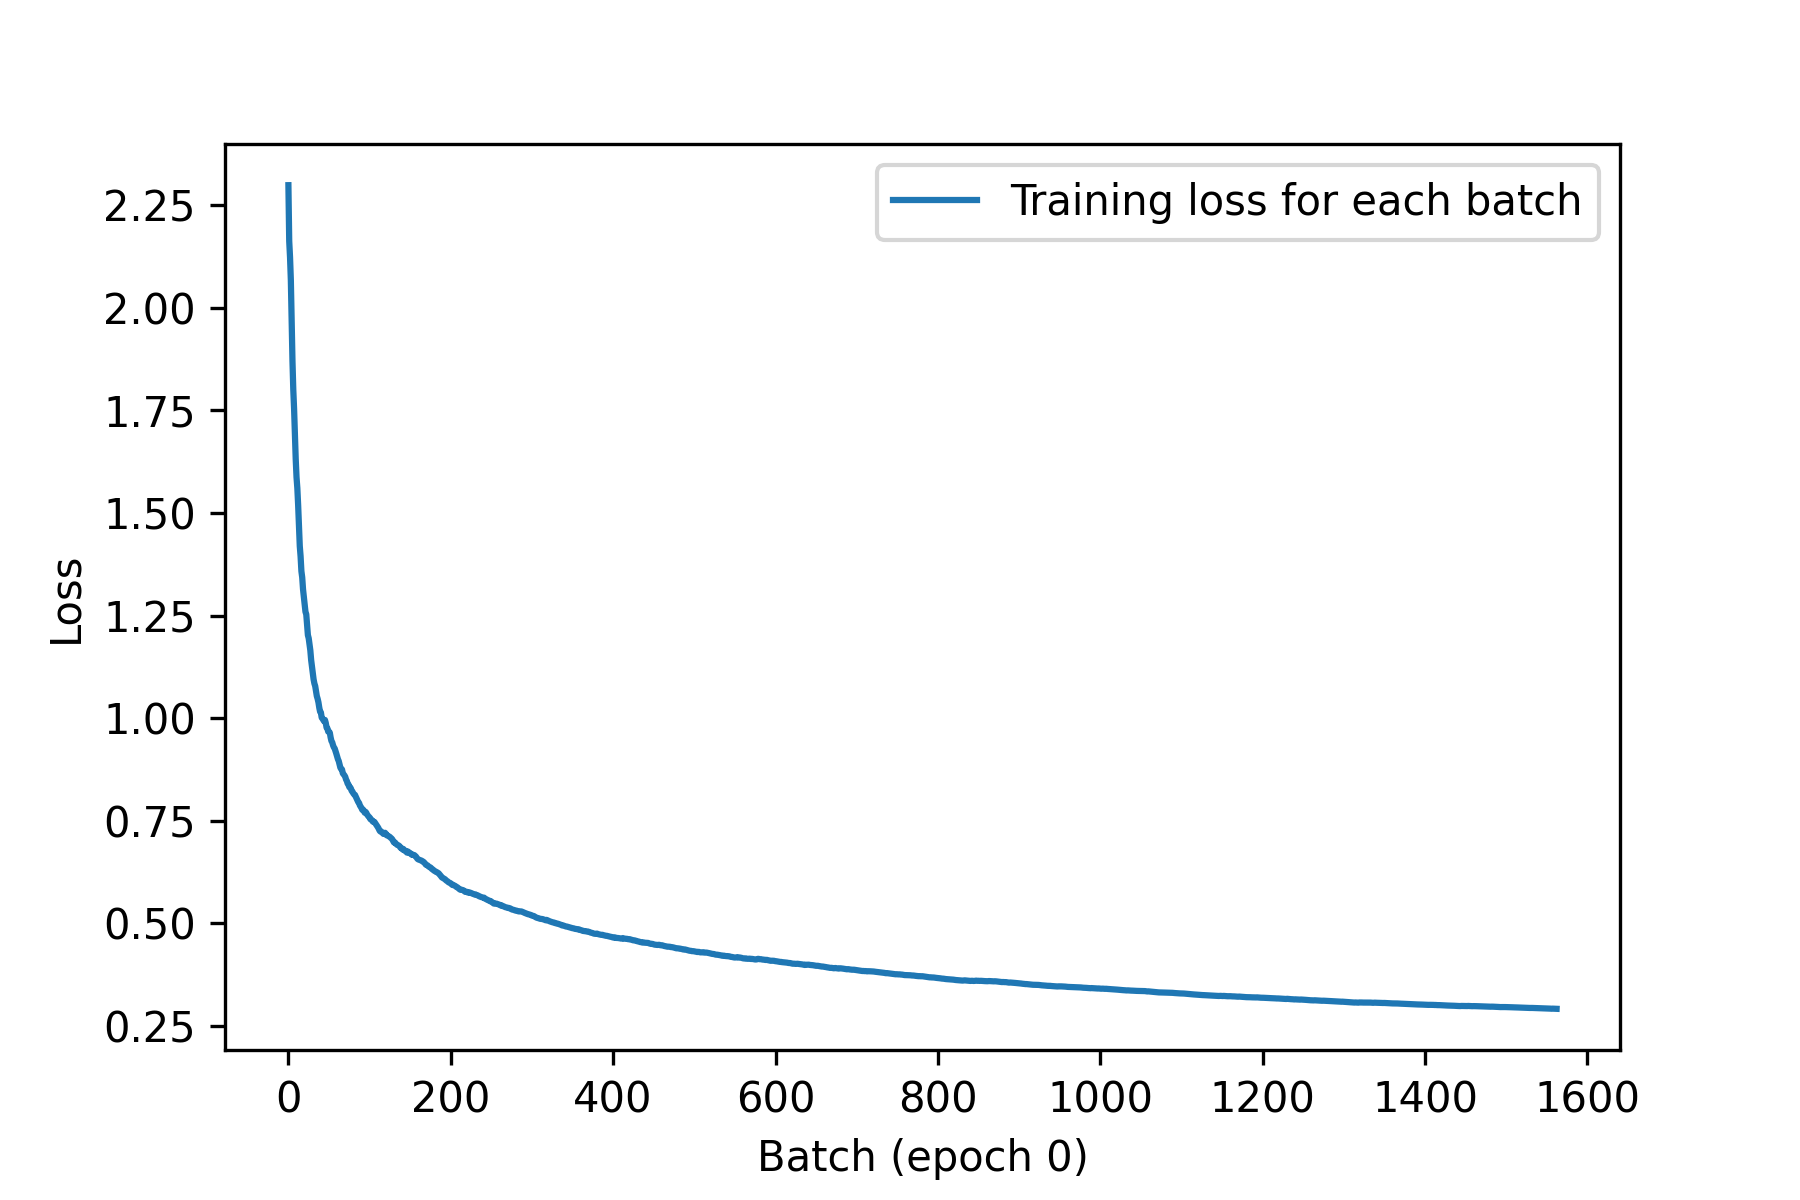
\includegraphics[width=\textwidth,height=0.7\textheight,keepaspectratio]{../../images/ch07/loss_history_callback_example.1e42f6b2.png}
            \caption{Đồ thị Loss sinh ra cuối quá trình}
        \end{figure}
    \end{columns}
\end{frame}

\section{5. Giám sát với TensorBoard}

\begin{frame}{Bảng điều khiển TensorBoard}
    \begin{columns}
        \column{0.5\textwidth}
        \begin{itemize}
            \item Mắt thường không thể đọc hàng triệu con số in trên Terminal.
            \item \textbf{TensorBoard} chạy một Web Server nội bộ (chạy trên localhost:6006), theo dõi và trực quan hóa thời gian thực (Real-time).
            \item Là công cụ chuẩn mực của giới chuyên gia để phân tích sâu hoạt động mạng.
        \end{itemize}
        
        \column{0.5\textwidth}
        \begin{figure}
            \centering
            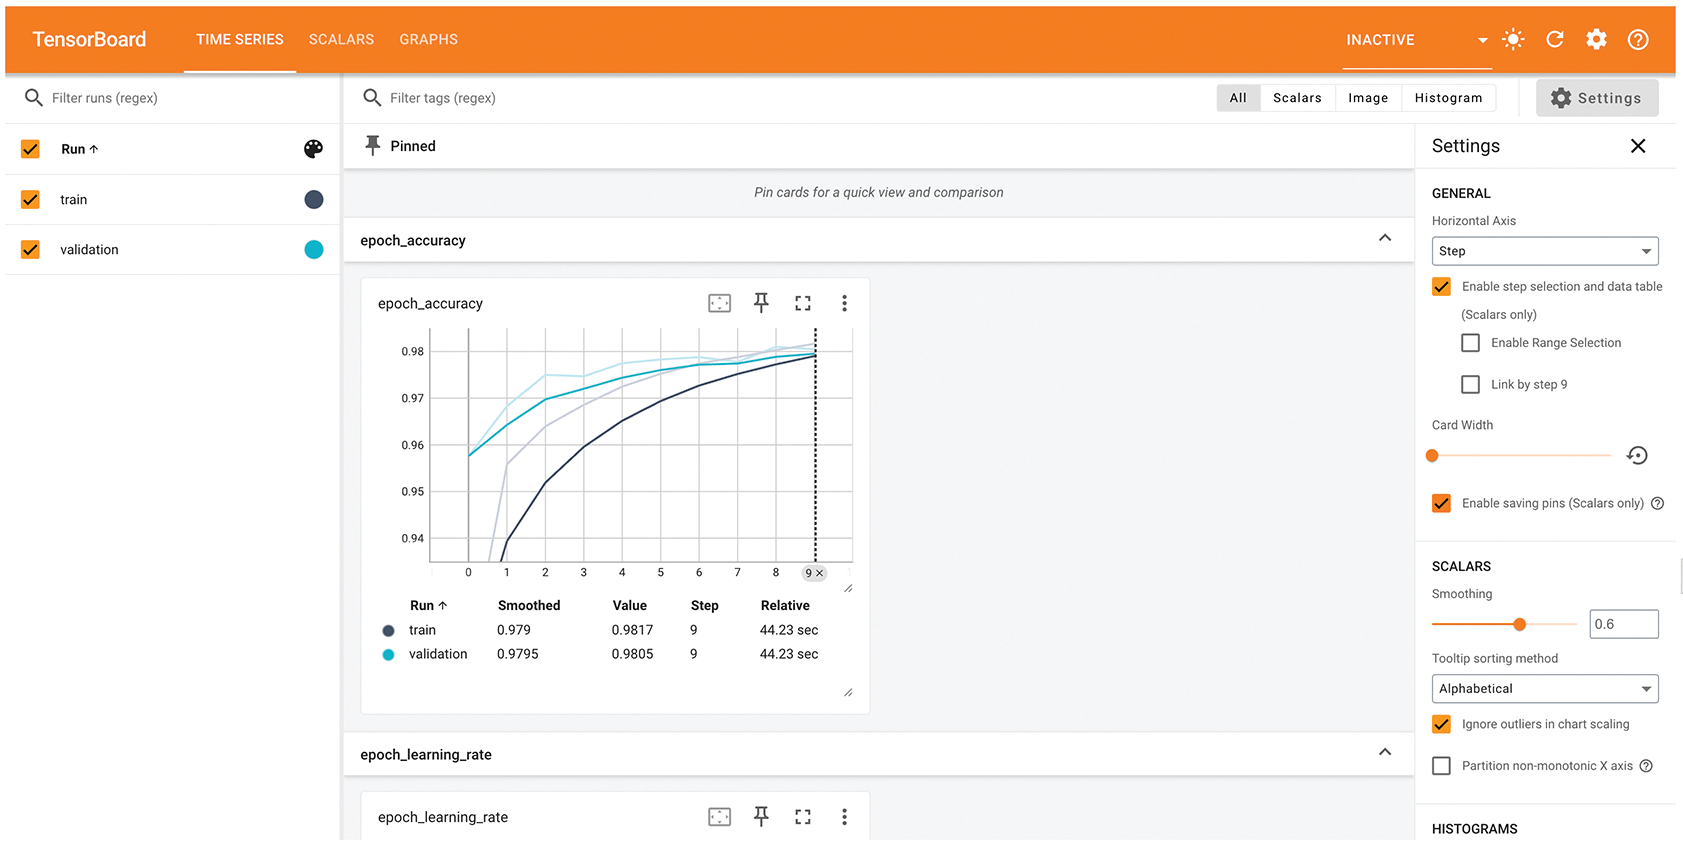
\includegraphics[width=\textwidth,height=0.7\textheight,keepaspectratio]{../../images/ch07/tensorboard.aec6cc75.png}
            \caption{Giao diện Giám sát TensorBoard}
        \end{figure}
    \end{columns}
\end{frame}

\begin{frame}[fragile]{Kích hoạt TensorBoard trong Keras}
Rất đơn giản, bạn chỉ cần dùng Callback \texttt{TensorBoard} có sẵn:

\begin{lstlisting}[language=Python]
callbacks = [
    keras.callbacks.TensorBoard(
        log_dir="/full_path_to_your_logs",
    )
]
model.fit(..., callbacks=callbacks)
\end{lstlisting}

Sau khi model chạy, mở Terminal và gọi:
\begin{lstlisting}[language=bash]
$ tensorboard --logdir /full_path_to_your_logs
\end{lstlisting}
Sau đó truy cập \texttt{http://localhost:6006} trên trình duyệt.
\end{frame}

\begin{frame}{Các tính năng cốt lõi của TensorBoard}
    \begin{itemize}
        \item \textbf{Metrics Viewer:} So sánh Metrics (Loss, Accuracy) của hàng chục thí nghiệm khác nhau cùng lúc (để Tune Hyperparameters).
        \item \textbf{Histograms:} Vẽ biểu đồ phân phối trọng số/kích hoạt để kiểm tra Gradient có bị Triệt tiêu (Vanishing) hay Bùng nổ (Exploding) hay không.
        \item \textbf{Graphs:} Vẽ lại Đồ thị Kiến trúc mô hình đa luồng.
        \item \textbf{Embeddings:} Chiếu (Project) không gian vector hàng ngàn chiều xuống 2D/3D (VD: PCA, t-SNE) để xem sự phân cụm của dữ liệu.
    \end{itemize}
\end{frame}

\section{Tổng kết}

\begin{frame}{Tổng kết Chương 7}
    Keras không chỉ là thư viện dành cho người mới, nó là một Vũ khí Chuyên sâu:
    \begin{itemize}
        \item Chọn đúng công cụ: 
        \begin{itemize}
            \item \textbf{Sequential}: Đơn giản (Mức 1).
            \item \textbf{Functional API}: Đa luồng đồ thị - Khuyên dùng hầu hết thời gian (Mức 2).
            \item \textbf{Model Subclassing}: Tự điều khiển luồng OOP (Mức 3).
        \end{itemize}
        \item Khả năng tùy biến vô hạn: Có thể tự viết lại \textbf{Custom Loss}, \textbf{Custom Metric}, và sử dụng \textbf{GradientTape} thay vì \texttt{fit()}.
    \end{itemize}
\end{frame}

\begin{frame}{Tổng kết Chương 7 (tiếp)}
    \begin{itemize}
        \item Giao thoa Workflow: Kết hợp Vòng lặp Tape thủ công bên trong hàm \texttt{train\_step()} để có ưu điểm của cả hai thế giới.
        \item Tự động hóa quá trình chạy thực nghiệm (Experiment) với hệ thống \textbf{Callbacks} (EarlyStopping, Checkpoint).
        \item Giám sát học thuật chuyên nghiệp: Trực quan hóa mọi thứ trực tuyến với Web Server \textbf{TensorBoard}.
    \end{itemize}
    \vspace{0.5cm}
    \textit{Bây giờ bạn đã đủ kiến thức để triển khai bất kỳ kỹ thuật học sâu phức tạp nào trong các chương tiếp theo!}
\end{frame}

\end{document}
